\chapter{Ecuaciones de variedades proyectivas}
\label{C3}

Nuestra tarea aquí es tratar de, dado un una recta o un plano proyectivos, dar una referencia proyectiva de ese subespacio mediante la cual hacer una descripción explícita de sus elementos.

\section{Rectas Proyectivas}\label{C3_sec_rectas}
\begin{defi}[Recta en $\proy(E)$]
	\label{C1_def_rectaProyectiva}
	Se define \ti{recta proyectiva} que pasa por los puntos proyetivos $P$ y $Q$ como la variedad engendrada por dichos puntos. A dicha recta se la denomina \ti{recta} $PQ$.
\end{defi}
\subsection{Ecuaciones paramétricas}\label{C3_subsec_ec_parametricas_recta}

Sean $P=\class{u}$ y $Q=\class{v}$ dos puntos proyectivos, vamos a describir los elementos de la recta $PQ$, que no es otra cosa que $\engen{P,Q}$.
	
Para describir los elementos de esta variedad (o de cualquiera) deberemos dar una referencia en función de la cual \ti{coordenar} todos los puntos de la misma.
	
Como $P$ y $Q$ son dos puntos proyectivos distintos, los vectores $u,v$ son linealmente independientes, formando una base de la variedad lineal $\lengen{u,v}$.
	
Para construir una referencia bastaría tomar los puntos $P,Q$ y añadirle como punto unidad un tercer punto cuyo representante pueda ser escrito como combinación lineal de $u$ y $v$ con todos los coeficientes no nulos, por ejemplo $\class{u+v}$.
	
De esta forma tenemos la referencia:
\[\mf{R}=\{P,Q;\class{u+v}\}\]
Por el método de construcción de bases asociadas tenemos que la base asociada a esta referencia es $\mc{B}=\{u,v\}$. Como sabemos, todo punto $p\in\engen{P,Q}$ es un rayo representado por un vector de $\lengen{u,v}$. Es decir, un vector $w=\alpha u+\beta v$ con alguno de los coeficientes no nulo.
	
Esto quiere decir que todo punto de la recta $PQ$ es un rayo de la forma: \[\class{\alpha u+\beta v}=(\alpha:\beta)\]
expresado en \ti{coordenadas homogéneas}.

Sin embargo, podemos reducir esto aún un poco más, cambiemos el representante del rayo dividiendo todo por $\beta$.
\[\class{\frac{\alpha}{\beta}u+v}:\stackrel{\textrm{not.}}{=}\class{\theta u+v}\]
De esta forma la recta ya no queda descrita por dos coordenadas homogéneas $\alpha$ y $\beta$ como antes, sino por una única coordenada $\theta$ a la que llamaremos \ti{no homogénea}.
	
Sin embargo, hemos de tener cuidado, pues, como más de uno ya se habrá dado cuenta, es posible que en algunos casos $\beta$ se anule, por ende, $\theta$ no estaría definida. Como este caso se corresponde con un único punto, y este es el punto $P$, diremos que una recta queda descrita por lo siguiente:
\begin{equation}
	\label{C3_eq_descripcionRecta}
	PQ:\{\class{\theta u+v}\tq \theta\in\K\}\cup\{P\}
\end{equation}
De esta forma, cuando $\beta=0$ podemos decir que $\theta=\infty$, y así $\theta\in\K\cup \{\infty\}$, que podemos identificar con $\proy^1$. Describiremos pues la recta como
\begin{equation}
	\label{C3_eq_descripcionRectaP1}
	PQ:\{\class{\theta u+v}\tq \theta\in\proy^1\}
\end{equation}
donde se entiende que si $\theta=\infty$ nos estamos refiriendo al punto $P$. 

Dados los vectores $u=(u_0,u_1,\cdots,u_n)$ y $v=(v_0,v_1,\cdots,v_n)$ si los sustituimos en la ecuación~\eqref{C3_eq_descripcionRectaP1} obtenemos
\begin{equation*}
	\label{C_3_eq_parametrica_recta}
	\begin{split}
		PQ:&\{\class{\theta (u_0,u_1,\cdots,u_n)+(v_0,v_1,\cdots,v_n)}\tq \theta\in\proy^1\}=\\
		&=\{\class{(\theta u_0+v_0,\theta u_1+v_1,\cdots,\theta u_n+v_n)}\tq \theta\in\proy^1\}
	\end{split}
\end{equation*}
que se puede escribir a su vez como 
\begin{equation}
	PQ:\{(\theta u_0+v_0:\theta u_1+v_1:\cdots:\theta u_n+v_n)\tq \theta\in\proy^1\}
\end{equation}
denominada \tb{ecuación paramétrica de la recta}, en coordenadas no homogéneas.
\begin{exa}[Parametrización de una Recta Concreta]
	\label{C3_exa_rectaConcreta}
	Dados los puntos $P=(1:2:-1)$ y $Q=(0:1:3)$ se nos pide parametrizar la recta $PQ$. Siguiendo los pasos expuestos en este apartado, la ecuación paramétrica de la recta $PQ$ queda:
	\[
	PQ:\{(\theta:2\theta+1:-\theta+3)\tq\theta\in\proy^1\}
	\]
	donde, cuando $\theta=\infty$, nos referimos al punto $P=(1:2:-1)$.
\end{exa}

\subsection{Ecuación implícita}\label{C3_subsec_eq_param_recta}

Durante este apartado nos situaremos en el plano proyectivo $\proy^2$, donde las rectas son hiperplanos. Como ya sabemos, todo hiperplano proyectivo es proyección de un hiperplano vectorial. Por tanto, una recta de $\proy^2$ es proyección de un plano de $\R^3$.

Además, por ser hiperplano, este plano tiene una, y solo una, ecuación implícita (o cartesiana) que cumplen todos sus vectores. Por tanto, todos los representantes de los puntos de la recta proyectiva cumplen dicha ecuación, ya que son los vectores del plano o sus múltiplos. 

De esta forma, asignamos a la recta de $\proy^2$ la ecuación implícita del plano vectorial del que es proyección
\begin{equation}
	\label{C3_eq_implicita_recta}
	ax+by+cz=0
\end{equation}
con $a,b,c$ no todos nulos. Esta será la \tb{ecuación implicita} de la recta, expresada en coordenadas homogéneas.

Veamos a continuación varias formas de obtener la ecuación implícita, en coordenadas homogéneas, de una recta proyectiva que pasa por dos puntos.

Sean $P=[u]=[(u_0,u_1,u_2)]$ y $Q=[v]=[(v_0,v_1,v_2)]$ dos puntos de $\proy^2$. La ecuación implícita de la recta $PQ$ tendrá la forma
\begin{equation*}
	ax+by+cz=0
\end{equation*}
donde $a,b,c$ son coeficientes a determinar.

Dado que $P,Q\in PQ$, la primera forma de hallar esos coeficientes consiste simplemente en sustituir en $x,y,z$ de la ecuación implícita las coordenadas de un vector representante de $P$ y de uno de $Q$ y resolver el sistema de ecuaciones resultante:
\begin{equation}
\label{C3_eq_implicitas_evaluadas}
	\begin{split}
		au_0+bu_1+cu_2=0\\
		av_0+bv_1+cv_2=0
	\end{split}
\end{equation}

Sin embargo, este método puede resultar un poco tedioso. Observemos que, aunque en el espacio proyectivo no está definido el producto escalar, la primera ecuación del sistema podría identificarse con el producto escalar entre el vector $(a,b,c)$ y $(u_0,u_1,u_2)$. Al ser cero, esto implicaría que son perpendiculares. A partir de la segunda ecuación podemos deducir algo similar, que $(a,b,c)$ es perpendicular al vector $(v_0,v_1,v_2)$.

De esta forma, el vector que debemos hallar es perpendicular a $u$ y $v$. Por tanto, nos basta con hallar un vector perpendicular a ambos para determinar los coeficientes de la ecuación implícita, pues es única salvo múltiplos. Una forma rápida de hallar un vector $(a,b,c)$ que cumpla esto es hacer el producto vectorial de $u$ y $v$. Así los coeficientes serán el resultado de 
\begin{equation}
	\label{C3_eq_implicita_cross_coef}
	(a,b,c)=u\times v=\left| \begin{array}{ccc}
		x & y & z\\
		u_0 & u_1 & u_2\\
		v_0 & v_1 & v_2
	\end{array}\right| 
\end{equation}
por lo que la ecuación implícita de la recta vendrá dada por 
\begin{equation}
\label{C3_eq_implicita_cross}
	(u\times v)\left( \begin{array}{c}
	x\\
	y\\
	z
	\end{array}\right) =0
\end{equation}
\subsection{Intersección de dos rectas proyectivas}
Una vez que sabemos describir una recta proyectiva a través de sus ecuaciones, no está de menos calcular la intersección de dos rectas. Para ello, nos situamos de nuevo en el plano proyectivo $\proy^2$, debido a la facilidad con la que allí se opera, pero bien sería válido para cualquier espacio proyectivo.

Sean pues dos rectas proyectivas $r,r'\in\proy^2$. Al igual que con la ecuación implícita de la recta, quizás la primera ocurrencia para hallar la intersección de dos rectas sea combinar sus ecuaciones implícitas y resolver el sistema resultante
\begin{equation*}
	\begin{split}
		ax&+by+cz=0\\
		a'x&+b'y+c'z=0
	\end{split}
\end{equation*}
donde $a,b,c,a',b',c'$ son conocidos.

Sin embargo, este método no es del todo práctico. Si nos paramos a reflexionar un momento sobre que debe cumplir la intersección, hallaremos formas mucho más fáciles de calcularla. Para empezar la intersección de $r$ y $r'$ es un punto $p$ del espacio proyectivo. Esto se debe a que en $\proy^2$ los hiperplanos son rectas, y por tanto, por el Corolario~\ref{C1_cor_rectaHiperplano}, la intersección de $r$ y $r'$ no puede ser vacía. Además, dicho punto pertenece tanto a $r$, como a $r'$. Por tanto, debe cumplir las ecuaciones de ambas rectas. Estas ecuaciones pueden ser tanto paramétricas como implícitas.

Si, por ejemplo, la recta $r$ está descrita a través de su ecuación paramétrica, donde $[(u_0,u_1,u_2)]$ y $[(v_0,v_1,v_2)]$ son dos puntos de la recta
\begin{equation*}
	r:\{(\theta u_0+v_0:\theta u_1+v_1:\theta u_2+v_2)\tq \theta\in\proy^1\}
\end{equation*}
existirá un valor de $\theta$ tal que 
\begin{equation}
\label{C3_eq_interseccion_rectas_imp_par}
	(\theta u_0+v_0:\theta u_1+v_1:\theta u_2+v_2)=p
\end{equation}
Una vez hallado ese valor, queda hallado el punto $p$ y con ello la intersección de ambas rectas.

Si, por otro lado, la recta $r'$ se describe a través de su ecuación implícita
\begin{equation*}
	a'x+b'y+c'z=0
\end{equation*}
el punto $p$ debe satisfacer dicha ecuación. Por tanto, podemos sustituir en la ecuación implícita de $r'$, en vez de las coordenadas de un representante arbitrario del punto $p$, las del vector\\
$(\theta u_0+v_0,\theta u_1+v_1,\theta u_2+v_2)$. Así, resolviendo la ecuación 
\begin{equation*}
 	a'(\theta u_0+v_0)+b'(\theta u_1+v_1)+c'(\theta u_2+v_2)=0
\end{equation*}
obtenemos el valor de $\theta$ que asegura que el punto $p$, descrito por la ecuación~\eqref{C3_eq_interseccion_rectas_imp_par} pertenece a ambas rectas. Sustituyendo este valor en la ecuación~\eqref{C3_eq_interseccion_rectas_imp_par} queda hallada la intersección de las rectas $r$ y $r'$.

Supongamos ahora que ambas rectas vienen descritas por su ecuación implícita. Al ser la intersección un punto $p=(p_0:p_1:p_2)$, podemos escoger un vector representante, por ejemplo $(p_0,p_1,p_2)$, y sustituirlo en ambas ecuaciones de tal forma que ambas deben cumplirse
\begin{equation*}
	\begin{split}
		ap_0&+bp_1+cp_2=0\\
		a'p_0&+b'p_1+c'p_2=0
	\end{split}
\end{equation*}
donde $p_0,p_1,p_2$ son desconocidos.

Detengámonos un segundo y observemos la ecuación~\eqref{C3_eq_implicitas_evaluadas}. ¿No se aprecia cierta similitud?. En efecto, en este caso el vector $(p_0,p_1,p_2)$ hace el papel de $(a,b,c)$. Si hacemos la misma interpretación, aunque no del todo correcta, de perpendicularidad a través del producto escalar, podemos afirmar que el vector que buscamos es perpendicular a los vectores $\vec{a}=(a,b,c)$ y $\vec{a}'=(a',b',c')$. Al igual que hicimos anteriormente, una forma rápida de hallar un vector perpendicular a otros dos, es hacer su producto vectorial. Por tanto, un vector representante del punto $p$ viene dado por
\begin{equation*}
	(p_0,p_1,p_2)=\vec{a}\times \vec{a}'=\left| \begin{array}{ccc}
		x & y & z\\
		a & b & c\\
		a' & b' & c'
	\end{array}\right| 
\end{equation*}
Es decir, la intersección de las rectas $r$ y $r'$ es el punto 
\begin{equation}
	p=[(p_0,p_1,p_2)]=[\vec{a}\times \vec{a}']
\end{equation}
Es importante observar que para encontrar el punto de corte entre dos rectas de $\proy^2$ se realiza la misma operación que para hallar los coeficientes de la ecuación implícita de la recta engendrada por dos puntos, correspondiente a la ecuación~\eqref{C3_eq_implicita_cross_coef}. 

\section{Planos Proyectivos}\label{C3_sec_planos}

Una vez completada la descripción de una recta, pasemos a realizar la de un plano de $\proy^3$. Este no es más que una variedad proyectiva de dimensión dos. Hallaremos sus ecuaciones paramétricas e implícitas generalizando los procedimientos del apartado anterior.

\subsection{Ecuaciones paramétricas}

Dados tres puntos proyectivos dis
tintos $P=[u]$, $Q=[v]$ y $S=[s]$, vamos a describir lo elementos del plano engendrado por ellos, es decir, los elementos de $\engen{P,Q,S}$. 

Para ello, y al igual que se hizo en el caso de la recta, debemos dar una referencia en función de la cual \ti{coordenar} los puntos de la variedad. Dado que los tres puntos $P,Q$ y $S$ son distintos, los vectores $u,v$ y $s$ son linealmente independientes, por lo que forman una base de $\lengen{u,v,s}$.

Así, utilizando el mismo razonamiento que en el apartado~\ref{C3_subsec_ec_parametricas_recta}, tomamos la referencia proyectiva dada por
\[\mf{R}=\{P,Q,S;\class{u+v+s}\}\]
cuya base asociada es $\mc{B}=\{u,v,s\}$.

Todo punto $p$ perteneciente al plano $\engen{P,Q,S}$ es un rayo representado por un vector $w$ de $\lengen{u,v,s}$. Por tanto, este vector puede ser escrito como $w=\alpha u +\beta v+\mu s$, con alguno de los coeficientes no nulo. Esto implica que los puntos del plano $\engen{P,Q,S}$, expresados en coordenadas homogéneas, tienen la forma
\[\class{\alpha u+\beta v+\mu s}=(\alpha:\beta:\mu)\]
Al igual que en el caso de la recta proyectiva, podemos reducir la expresión del plano y reescribirlo en función de dos coordenadas no homogéneas $\theta$ y $\gamma$:
\[\class{u+\frac{\beta}{\alpha}v+\frac{\mu}{\alpha}s}:\stackrel{\textrm{not.}}{=}\class{u+\theta v+\gamma s}\]
Sin embargo, en este caso, debemos tener más cuidado con los problemas que surgen cuando $\alpha=0$.

Si $\alpha=0$ y $\beta\not=0\not=\mu$, entonces estaremos haciendo referencia al punto $[v+s]$. En este caso diremos que $\theta=\infty=\gamma$. Por otro lado, si $\alpha=0$ y $\beta=0$, entonces el punto resultante se corresponde con $S$, y diremos que esto se da cuando $\gamma=\infty$. Asimismo, cuando $\theta=\infty$, estamos haciendo referencia al punto $Q$.

Teniendo en cuenta estas indeterminaciones, el plano $\engen{P,Q,S}$ puede describirse a través de
\begin{equation}
\label{C3_eq_descripcionPlanoP1}
\engen{P,Q,S}:\{\class{u+\theta v+\gamma s}\tq \theta,\gamma\in\proy^1\}
\end{equation}
siendo esta la \tb{ecuación paramétrica del plano}, en coordenadas no homogéneas.

\begin{obs}
	Este procedimiento para hallar las ecuaciones paramétricas de un plano de $\proy^3$ no es más que una adaptación del procedimiento que se llevó a cabo en el apartado~\ref{C3_subsec_ec_parametricas_recta}. Observemos que es un procedimiento fácilmente generalizable a cualquier variedad proyectiva, sea cual sea su dimensión y la del espacio proyectivo. Por tanto, no se explicará como hallar las ecuaciones paramétricas de una variedad proyectiva general, pues basta seguir los pasos del apartado~\ref{C3_subsec_ec_parametricas_recta}, adaptándolo a las dimensiones de su caso.
\end{obs}

\subsection{Ecuación implícita}

Dado que un plano en $\proy^3$ es un hiperplano, al igual que ocurría con la recta en $\proy^2$ y siguiendo el mismo razonamiento, le asignaremos la ecuación implícita del hiperplano de $\R^4$ del que es proyección
\begin{equation}
\label{C3_eq_implicita_plano}
ax+by+cz+dt=0
\end{equation}
con los coeficientes no todos nulos. Esta será la \tb{ecuación implicita} del plano, expresada en coordenadas homogéneas. 

Dados tres puntos proyectivos $P=[(u_0,u_1,u_2,u_3)]$, $Q=[(v_0,v_1,v_2,v_3)]$ y $S=[(s_0,s_1,s_2,s_3)]$ de $\proy^3$, desarrollemos un procedimiento para hallar la ecuación implícita del plano que engendran $\engen{P,Q,S}$. Al igual que con la ecuación paramétrica, no haremos más que adaptar el apartado~\ref{C3_subsec_eq_param_recta} a nuestro caso.

Recordemos que la primera forma de hacer esto que se comentó era, dado que $P,Q,S\in \engen{P,Q,S}$, sustituir en la ecuación~\eqref{C3_eq_implicita_plano} las coordenadas de vectores representantes de los tres puntos proyectivos y resolver el sistema. Sin embargo, no era la más eficaz.
\begin{equation}
	\begin{split}
		au_0+bu_1+cu_2+du_3=0\\
		av_0+bv_1+cv_2+dv_3=0\\
		as_0+bs_1+cs_2+ds_3=0
	\end{split}
\end{equation}
Otra forma, bastante mejor que la anterior, era interpretar las ecuaciones anteriores como el producto escalar entre el vector $(a,b,c,d)$ y los vectores representantes de los puntos $P,Q$ y $S$. Esto en la recta nos llevaba a un producto vectorial. Sin embargo, en $\R^4$ no está definido. Por tanto, debemos darle a las ecuaciones otra interpretación, para así hallar una forma más fácil de calcular la ecuación implícita de un plano. 

Por un momento, observemos la eucación~\eqref{C3_eq_implicita_plano} como la ecuación implícita del hiperplano $H$ cuya proyección es el plano proyectivo $\engen{P,Q,S}$. Si consideramos $x,y,z$ y $t$ como coordenadas de un punto de $H$, dado que los vectores $u,v,t$ forman una base de dicho plano, como se explicó en el apartado anterior, el vector $(x,y,z,t)$ será combinación lineal de ellos, y por tanto el conjunto $\{(x,y,z,t),u,v,s\}$ será linealmente dependiente. Con ello el determinante
\begin{equation}
	\left| \begin{array}{cccc}
	x & y & z& t\\
	u_0 & u_1 & u_2 & u_3\\
	v_0 & v_1 & v_2 & v_3\\
	s_0 & s_1 & s_2 & s_3
	\end{array}\right| =0
\end{equation}
debe ser nulo. De esta forma, dado que las únicas incógnitas con $x,y,z$ y $t$ y la ecuación implícita es única salvo múltiplos, el resultado de ese determinante será la ecuación implícita del hiperplano $H$, que por definición es la ecuación implícita del plano proyectivo $\engen{P,Q,S}$.

\begin{obs}
	Aunque el procedimiento utilizado para calcular la ecuación implícita de una recta de $\proy^2$ a través del producto vectorial no es generalizable a otros hiperplanos, como acabamos de ver, el desarrollado en este apartado sí lo es. Por ello, no se explicará como hallar la ecuación implícita de un hiperplano proyectivo general, ya que bastará con seguir los pasos de esta sección, adaptándolos a las dimensiones pertinentes. Esto implica evidentemente, que la ecuación implícita de una recta de $\proy^2$ se puede hallar también a través de este procedimiento.
\end{obs}

\section{Haz de hiperplanos}
En este apartado retomaremos el espacio proyectivo dual y le daremos otra utilidad, que nos será de gran ayuda a la hora de calcular intersecciones de hiperplanos.

\subsection{Haz de rectas}
Por el momento, dado que es mucho más intuitivo explicar el concepto  con hiperplanos concretos, empezaremos trabajando con rectas en $\proy^2$.
\begin{defi}
	Dado un punto $p\in\proy^2$, se define el \ti{haz de rectas} por el punto $p$, o con base $p$, al conjunto de todas las rectas de $\proy^2$ que pasan por $p$.
\end{defi}
Observemos que dos cualesquiera rectas de este haz generan el plano proyectivo. Por tanto dadas tres rectas del haz con ecuaciones implícitas
\begin{equation}
	\label{C3_eq_implicitas_rectas_haz}
	\begin{split}
		r:a_0x+a_1y+a_2z=0\\
		r':b_0x+b_1y+b_2z=0\\
		r'':c_0x+c_1y+c_2z=0
	\end{split}
\end{equation}
los sistemas de ecuaciones 
\begin{equation}
	\begin{cases}
	a_0x+a_1y+a_2z=0\\
	b_0x+b_1y+b_2z=0
	\end{cases} \qquad \text{y} \qquad \begin{cases}
	a_0x+a_1y+a_2z=0\\
	b_0x+b_1y+b_2z=0\\
	c_0x+c_1y+c_2z=0
	\end{cases}
\end{equation}
son equivalentes. Esto implica que una de las ecuaciones es combinación lineal de las otras dos. Por tanto, conocidas dos rectas del haz $r$ y $r'$, la ecuación implícita en coordenadas homogéneas de cualquiera otra recta del haz vendrá dada por
\begin{equation}
	\label{C3_eq_recta_haz}
	\alpha(a_0x+a_1y+a_2z)+\beta(b_0x+b_1y+b_2z)=0
\end{equation}
para determinados $\alpha$ y $\beta$. Si $\alpha\not=0$ podemos dividir por él, y la ecuación quedaría
\begin{equation}
	\label{C3_eq_recta_haz_nohom}
	(a_0x+a_1y+a_2z)+\theta(b_0x+b_1y+b_2z)=0\tq \theta=\frac{\beta}{\alpha}
\end{equation}
en coordenadas no homogéneas. 

Así, si dadas dos rectas del haz queremos determinar otra recta $s$ que pase por un punto $q$, distinto del punto $p$ del haz, basta sustituir las coordenadas de un vector representante de dicho punto $q$ que la ecuación~\eqref{C3_eq_recta_haz_nohom}, obteniendo así un valor de $\theta$. Sustituyendo $\theta$ de nuevo en la ecuación~\eqref{C3_eq_recta_haz_nohom} obtenemos la ecuación implícita de $s$.\\

Sin embargo, un haz de rectas admite una interpretación dual, que da mucho más juego. Veremos que lo obtenido sin el espacio proyectivo dual es compatible con lo que obtendremos a partir de él.

Recordando el principio de dualidad, \ti{traduzcamos} la definición de haz de rectas. De esta forma, y dado que estamos en $\proy^2$, los puntos pasan a ser rectas, y las rectas, puntos. Por tanto, todas las rectas que se cortan en el punto $p$ son todos los puntos que engendran la recta dual $p^*$. Con ello, todo haz de rectas con base $p$ de $\proy^2$ representa una recta $p^*$ en el dual. Asimismo, gracias a la dualidad, toda recta $p^*$ de $\proy^{2^*}$ representa un haz de rectas con base $p$ en $\proy^2$.

Por tanto, un haz de rectas $p^*$ es una variedad proyectiva dual de dimensión 1, engendrada por dos puntos duales
\begin{equation}
	p^*:=\{\proy(\lengen{r,r'})\tq r,r'\text{ son puntos de }\proy^{2^*}\}
\end{equation}
Estos puntos son rectas en el espacio proyectivo $\proy^2$, por lo que tienen una ecuación implícita
\begin{equation*}
	a_0x+a_1y+a_2z=0
\end{equation*}
Así, las coordenadas de una recta en el espacio proyectivo dual serán $(a_0:a_1:a_2)$. Por tanto, si se conocen dos rectas del haz, se conocen dos puntos del haz $p^*$, y podemos describirlo a través de ecuaciones paramétricas e implícitas. 

Esta descripción es la misma que la realizada en el apartado~\ref{C3_sec_rectas}, ya que al fin y al cabo se trata de describir una recta a partir de dos puntos, aunque todo ello se desarrolle en el espacio proyectivo dual. 

Sean pues dos rectas $r$ y $r'$ del haz de rectas en $\proy^2$. Estas, por la ecuación~\eqref{C3_eq_implicitas_rectas_haz}, representan los puntos $(a_0:a_1:a_2)$ y $(b_0:b_1:b_2)$ en $\proy^{2^*}$. La ecuación paramétrica del haz de rectas, o recta dual $p^*$, es, en coordenadas homogéneas
\begin{equation}
	p^*:\{\class{\alpha (a_0,a_1,a_2)+\beta (b_0,b_1,b_2)\tq \alpha,\beta\in\R}\}
\end{equation}
En coordenadas no homogéneas adopta la forma
\begin{equation}
p^*:\{\class{(a_0,a_1,a_2)+\theta (b_0,b_1,b_2)}\tq \theta\in\proy^1\}=\{(a_0+\theta b_0:a_1+\theta b_1:a_2+\theta b_2)\tq \theta\in\proy^1\}
\end{equation}
Hagamos una rápida comprobación de que esto es coherente con lo explicado al principio de este apartado, sin tener en cuenta la dualidad. 

Los punto que pertenecen al haz de rectas $p^*$ en el dual son aquellos de la forma\\
$(a_0+\theta b_0:a_1+\theta b_1:a_2+\theta b_2)$. Es decir, traduciendo de nuevo, aquellas rectas de $\proy^2$ cuya ecuación implícita es
\begin{equation*}
	(a_0+\theta b_0)x+(a_1+\theta b_1)y+(a_2+\theta b_2)z=0
\end{equation*}
son las que pertenecen al haz de rectas de $\proy^2$. Observamos que esta ecuación coincide con la ecuación~\eqref{C3_eq_recta_haz_nohom}, con la cual también habíamos deducido que todas las rectas del haz debían tener por ecuación implícita la ecuación~\eqref{C3_eq_recta_haz_nohom}. Por tanto, ambas representaciones coinciden.

Por último, hallemos la ecuación implícita de $p^*$. Guiándonos por el apartado~\ref{C3_sec_rectas} de nuevo, tenemos que la ecuación implícita de una recta, conocidos dos de sus puntos, es 
\begin{equation}
((a_0,a_1,a_2)\times(b_0,b_1,b_2))\left( \begin{array}{c}
u\\
v\\
w
\end{array}\right) =0
\end{equation}
O bien, a partir del apartado~\ref{C3_sec_planos}
\begin{equation}
	\label{C3_eq_implicita_rectadual_determinante}
	\left| \begin{array}{ccc}
	u & v & w \\
	a_0 & a_1 & a_2\\
	b_0 & b_1 & b_2
	\end{array}\right| =0
\end{equation}
Nótese que, en vez de llamar a las variables $x,y, z$, las hemos llamado $u,v,w$, para no confundir ecuaciones de rectas proyectivas con ecuaciones de rectas proyectivas duales.

\begin{obs}
	Es importante observar que, por el mismo procedimiento, se puede describir una recta de $\proy^2$ o una de $\proy^{2^*}$. La única diferencia es si consideramos los coeficientes de una ecuación como coordenadas de un punto o como coeficientes de una recta.
\end{obs}

\subsubsection{Intersección de dos rectas proyectivas}
Anteriormente hemos estudiado varias formas de calcular la intersección de dos rectas de $\proy^2$. Sin embargo, el concepto de haz de rectas aun no había sido introducido. Una vez conocida su existencia, utilicémoslo para hallar la intersección de dos rectas $r$ y $r'$ en $\proy^2$, descritas por las siguientes ecuaciones implícitas
\begin{equation*}
	\begin{split}
		r:a_0x+a_1y+a_2z=0\\
		r':b_0x+b_1y+b_2z=0
	\end{split}
\end{equation*}
Como bien sabemos, dicha intersección es un punto $p=(p_0:p_1:p_2)$. Esto quiere decir que las dos rectas $r$ y $r'$ pertenecen al haz de rectas con base $p$. 

Pasando al espacio dual estamos buscando una recta $p^*$ de $\proy^{2^*}$, con ecuación implícita
\begin{equation}
	\label{C3_eq_ejemplo_int_rectas_dual}
	p_0u+p_1v+p_2w=0
\end{equation}
que contiene a los puntos $(a_0:a_1:a_2)$ y $(b_0:b_1:b_2)$. 

La ecuación implícita de una recta que pasa por dos puntos viene dada por la ecuación~\eqref{C3_eq_implicita_rectadual_determinante}. Sustituyendo los valores de los puntos contenidos en $p^*$ obtenemos
\begin{equation*}
	\left| \begin{array}{ccc}
	u & v & w \\
	a_0 & a_1 & a_2\\
	b_0 & b_1 & b_2
	\end{array}\right| =0
\end{equation*}
\begin{equation*}
	(a_1b_2-a_2b_1)u+(a_2b_0-a_0b_2)v+(a_0b_1-a_1b_0)w=0
\end{equation*}
que se corresponde a la ecuación implícita de la recta dual $p^*$. Comparando con la eucación~\eqref{C3_eq_ejemplo_int_rectas_dual} obtenemos que la intersección de las rectas $r$ y $r'$ de $\proy^2$ es el punto
\begin{equation*}
	p=(a_1b_2-a_2b_1:a_2b_0-a_0b_2:a_0b_1-a_1b_0)
\end{equation*}
\subsection{Haz de hiperplanos}
El concepto de haz de rectas puede generalizarse a un espacio proyectivo $\proy(E)$, siempre que se considere un conjunto de hiperplanos. Hagamos una definición general.
\begin{defi}
	Se llama haz de hiperplanos al conjunto de todos los hiperplanos de $\proy(E)$ que contienen una variedad proyectiva dada $X\subset\proy(E)$ de codimensión $2$. Esa variedad $X$ se llama base del haz.
\end{defi}
Por ejemplo, en $\proy^3$, estaríamos hablando de un haz de planos con base la recta $r$ por la cual pasan todos ellos.

Dado que se habla de haz de hiperplanos, estos vendrán descritos por una ecuación implícita. Por tanto, todas las explicaciones realizadas en el apartado anterior basándonos en las ecuaciones implícitas, sin usar el dual, son válidas para el caso general.

Además, la interpretación dual sigue correcta. Cada hiperplano de $\proy(E)$ es un punto en el espacio proyectivo dual. La variedad $X$ contenida en todos ellos, dado que tiene codimensión $2$, es una recta en $\proy^*$. Por tanto, todo haz de hiperplanos con base $X$ de $\proy(E)$ representa una recta $X^*$ en el dual. De forma general, un haz de hiperplanos es una variedad proyectiva dual de dimensión $1$. 

Al igual que hicimos en el apartado anterior, podemos describir el haz de hiperplanos $X^*$, dado que es una recta del dual, a través de sus ecuaciones paramétricas. Dados dos hiperplanos del haz, tenemos dos puntos de $X^*$ conocidos. Así, se reduce a hallar al ecuación implícita de una recta que pasa por dos puntos, problema descrito en la sección~\ref{C3_subsec_ec_parametricas_recta}.

\section{Teorema de Pappus}
En esta sección enunciaremos un teorema clásico de la geometría del plano proyectivo, en cuya demostración usaremos lo visto a lo largo de este capítulo.
\begin{theo}[Teorema de Pappus]
	Sea $\proy(E)$ un plano proyectivo y sean $r$ y $r'$ dos rectas diferentes de $\proy(E)$. Entonces, para cualesquiera seis puntos distintos $A,B,C\in r$ y $A',B',C'\in r'$, los puntos
	\begin{equation*}
		X=AB'\cap A'B \ ; \qquad Y=AC'\cap A'C \ ; \qquad Z=BC'\cap B'C
	\end{equation*}
	están alineados.
\end{theo}
\begin{center}
	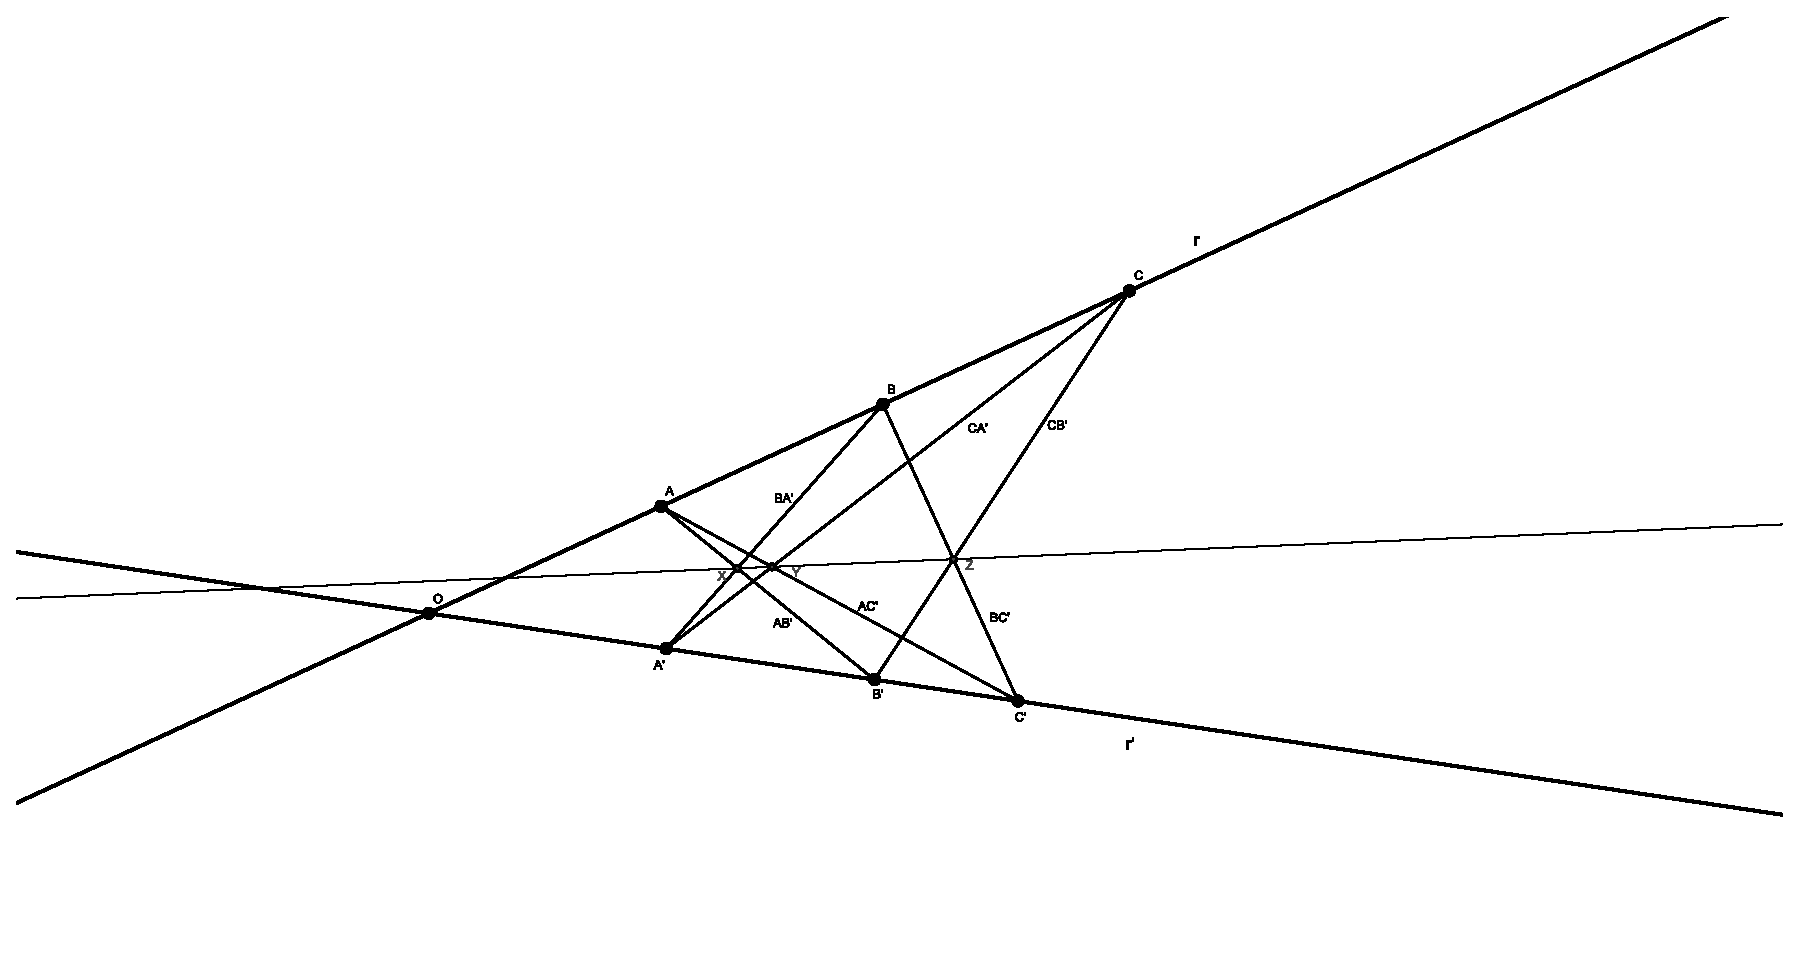
\includegraphics[scale=.5]{Graficos/TeoremaDePapus/Teorema_Papus.eps}
\end{center}
\begin{proof}
	Dado que en el plano proyectivo las rectas son hiperplanos, y haciendo uso del corolario~\ref{C1_cor_rectaHiperplano}, las rectas $r$ y $r'$ se cortan en un punto $O$. 
	
	Si alguno de los seis puntos es $O$, el teorema es trivial ya que dos de los puntos $X,Y$ y $Z$ coincidirían, con lo que tendríamos dos puntos trivialmente alineados. Trataremos pues el caso en que todos ellos son diferentes de $O$.
	
	La demostración consistirá en hallar las coordenadas de los puntos $X,Y,Z$ y comprobar que están alineados. Para ello es necesario establecer una referencia proyectiva. Por comodidad elegimos
	\begin{equation*}
		\mf{R}=\{A,B,C';B'\}
	\end{equation*}
	Comprobemos que es referencia. Por hipótesis, dado que son distintos, los puntos $A,B$ y $C'$ forman un triángulo no degenerado. Por tanto, para ver que cada $3$ de ellos son proyectivamente independientes, bastaría comprobar que el punto $B'$ no está en ninguno de los lados del triángulo $ABC'$.
	
	Dado que $B'\in r'\smz$ es claro que no pertenece a la recta $AB=r$. Tampoco está en $AC'$ ya que, en caso contrario, $B'\in r'\cap AC'=\{C'\}$, lo cual es absurdo pues los puntos $B'$ y $C'$ son distintos. Por último, no pertenece a $BC'$, pues en caso contrario de nuevo tendríamos que $B'\in r'\cap BC'=\{C'\}$. 
	
	Una vez demostrado que $\mf{R}$ es una referencia proyectiva, las coordenadas de los puntos $A,B,C'$ y $B'$ respecto a dicha referencia son
	\begin{equation*}
		A=(1:0:0) \ ; \qquad B=(0:1:0) \ ; \qquad C'=(0:0:1) \ ; \qquad B'=(1:1:1)
	\end{equation*}
	Estamos en situación de hallar las coordenadas de los puntos $X,Y$ y $Z$ respecto a la referencia $\mf{R}$. Realizaremos el mismo procedimiento para todos los puntos: hallaremos las ecuaciones, paramétricas o implícitas, de las rectas cuya intersección es el punto en cuestión, y a partir de ellas calcularemos posteriormente dicha intersección.
	\begin{itemize}
		\item Punto $X=AB'\cap A'B$.
		
		Dado que las coordenadas respecto a nuestra referencia de los puntos $A$ y $B'$ son conocidas, la ecuación implícita de la recta $AB'$ es
		\begin{equation*}
			\left| \begin{array}{ccc}
				x & y & z\\
				1 & 0 & 0\\
				1 & 1 & 1
			\end{array}\right| =0 \ \sii \ z-y=0
		\end{equation*}
		Para la recta $ A'B$ primero debemos hallar las coordenadas de $A'$ respecto de $\mf{R}$. Es un punto de $B'C'=r'$ distinto de $O,B',C'$. Las ecuaciones paramétricas de $B'C'$, tomando como representantes los vectores $(1,1,1)$ y $(0,0,1)$, son
		\begin{equation}
			\label{C3_papus_eqparam_r}
			r'=B'C':=\{[\lambda(1,1,1)+\mu(0,0,1)]\tq \lambda,\mu\in E\}=\{(\lambda:\lambda:\mu+\lambda)\tq \lambda,\mu\in E\}
		\end{equation}
		Por lo que $A'$ es un punto de la forma $(\lambda:\lambda:\mu+\lambda)$. Dado que no es el punto $C'$, $\lambda\not=0$, pudiendo así dividir por $\lambda$. Queda
		\begin{equation*}
			A'=(1:1:1+\frac{\mu}{\lambda})=(1:1:\theta)\tq \theta=1+\frac{\mu}{\lambda}
		\end{equation*}
		Tengamos en cuenta que como $A'\not=B'$, $\theta\not=1$. Además, $A'\not=O$ por lo que nos falta una restricción para $\theta$. Calculamos el punto $O$ para hallarla. La ecuación implícita de $r=AB$ es 
		\begin{equation*}
			\left| \begin{array}{ccc}
				x & y & z\\
				1 & 0 & 0\\
				0 & 1 & 0
			\end{array}\right| =0 \ \sii \ z=0
		\end{equation*}
		Con ello se obtiene que el punto de corte cumple $\mu=-\lambda$. Por tanto, la intersección de ambas rectas es el punto $(\lambda:\lambda:0)=(1:1:0)$. La restricción que debemos imponer a $\theta$ para que $A'\not=O$ es que $\theta\not=0$. Así
		\begin{equation*}
			A'=(1:1:\theta)\tq \theta=1+\frac{\mu}{\lambda}, \theta\not=0, \theta\not=1
		\end{equation*}
		La ecuación implícita de la recta $A'B$ es
		\begin{equation*}
			\left| \begin{array}{ccc}
				x & y & z\\
				1 & 1 & \theta\\
				0 & 1 & 0
			\end{array}\right| =0 \ \sii \ \theta x+z=0
		\end{equation*}
		Finalmente resolviendo el sistema 
		\begin{equation}
			\begin{split}
				AB':&z-y=0\\
				A'B:&\theta x+z=0
			\end{split}
		\end{equation}
		obtenemos el punto $X=AB'\cap A'B$
		\begin{equation}
			\label{C3_pappus_X}
			X=(1:\theta:\theta)
		\end{equation}
		
		\item Punto $Z=BC'\cap B'C$.
		
		La ecuación implícita de la recta $BC'$ es
		\begin{equation*}
			\left| \begin{array}{ccc}
				x & y & z\\
				0 & 1 & 0\\
				0 & 0 & 1
			\end{array}\right| =0 \ \sii \ x=0
		\end{equation*}
		Para describir la recta $B'C$ debemos hallar antes el punto $C$. Este se encuentra en la recta $AB$, que descrita a través de las ecuaciones paramétricas es
		\begin{equation*}
			AB:=\{[\alpha(1,0,0)+\beta(0,1,0)]\tq \alpha,\beta\in E\}=\{(\alpha:\beta:0)\tq \alpha,\beta\in E\}
		\end{equation*}
		Dado que $C\not=B$, se tiene que $\alpha\not=0$, por lo que podemos dividir por ella
		\begin{equation*}
			C=(1:\frac{\beta}{\alpha}:0)=(1:\mu:0)\tq \mu=\frac{\beta}{\alpha}
		\end{equation*}
		Por otro lado $C\not=O=(1:1:0)$, lo cual implica que $\mu\not=1$. Además $C\not=A$, por lo que $\mu\not=0$. Así, finalmente el punto $C$ es
		\begin{equation*}
			C=(1:\mu:0)\tq \mu=\frac{\beta}{\alpha},\mu\not=0,\mu\not=1
		\end{equation*}
		Ahora ya podemos calcular las ecuaciones paramétricas de la recta $B'C$, las cuales, en coordenadas no homogéneas, vienen dadas por
		\begin{equation*}
			B'C:=\{[(1,\mu,0)+\nu(1,1,1)]\tq \nu\in\proy^1\}=\{(1+\nu:\mu+\nu:\nu)\tq \nu\in\proy^1\}
		\end{equation*}
		El punto de intersección de las rectas $BC'$ y $B'C$ cumple $1+\nu=0$. Por tanto, $\nu=-1$ y la intersección de ambas es 
		\begin{equation}
			\label{C3_pappus_Z}
			Z=(0:\mu-1:-1)
		\end{equation}
		
		
		\item Punto $Y=AC'\cap A'C$.
		
		La ecuación implícita de la recta $AC'$ es
		\begin{equation*}
			\left| \begin{array}{ccc}
				x & y & z\\
				1 & 0 & 0\\
				0 & 0 & 1
			\end{array}\right| =0 \ \sii \ y=0
		\end{equation*}
		Por otro lado, las ecuaciones paramétricas de $A'C$, teniendo en cuenta las restricciones antes impuestas a $\theta$ y $\mu$, son
		\begin{equation*}
			A'C:=\{[(1,1,\theta)+\xi(1,\mu,0)]\tq \xi\in\proy^1\}=\{(1+\xi:1+\mu\xi:\theta)\tq \xi\in\proy^1\}
		\end{equation*}
		El punto de intersección de ambas rectas cumple $1+\mu\xi=0$, con lo cual $\xi=\frac{-1}{\mu}$. Finalmente el punto $Y$ es
		\begin{equation}
			\label{C3_pappus_Y}
			Y=(1-\frac{1}{\mu}:0:\theta)=(\mu-1:0:\mu\theta)
		\end{equation}
		
	\end{itemize}
	Una vez que tenemos las coordenadas de los tres puntos respecto a la referencia $\mf{R}$ falta comprobar que están alineados. Para ello, sus representantes deben ser coplanarios, es decir, su determinante debe ser nulo. Haciendo uso de las ecuaciones~\eqref{C3_pappus_X},~\eqref{C3_pappus_Y} y~\eqref{C3_pappus_Z} comprobamos que esto se cumple
	\begin{equation*}
		\left| \begin{array}{ccc}
			1 & \mu-1 & 0\\
			\theta & 0 & \mu-1\\
			\theta & \mu\theta & -1
		\end{array}\right| =(\mu-1)^2\theta-(\mu-1)\mu\theta+(\mu-1)\theta=\mu^2\theta+\theta-2\mu\theta-\mu^2\theta+2\mu\theta-\theta=0
	\end{equation*}
	Es importante observar que en general el determinante de los representantes de tres puntos proyectivos no está bien definido, debido a que podemos coger múltiplos. Sin embargo en este caso, al ser igual a cero, sí lo está. Por ello, el teorema queda demostrado.
\end{proof}
Recordemos que gracias al principio de dualidad, dado un teorema, automáticamente su dual es cierto. Así, podemos enunciar el Teorema de Pappus para el plano proyectivo dual y quedará demostrado, por el simple hecho de haber demostrado el teorema en el plano proyectivo.
\begin{theo}[Teorema de Pappus Dual]
	Sea $\proy(E^*)=\proy^*$ un plano proyectivo dual y sean $R$ y $R'$ dos puntos distintos de $\proy^*$. Entonces, para cualesquiera seis rectas distintas $a,b,c,a',b',c'$ tales que $R\in a,b,c$ y $R'\in a',b',c'$; las rectas
	\begin{equation*}
		\engen{a\cap b',a'\cap b} \ ; \qquad \engen{a\cap c',a'\cap c} \ ; \qquad \engen{b\cap c',b'\cap c}
	\end{equation*}
	son concurrentes.
\end{theo}
\begin{center}
	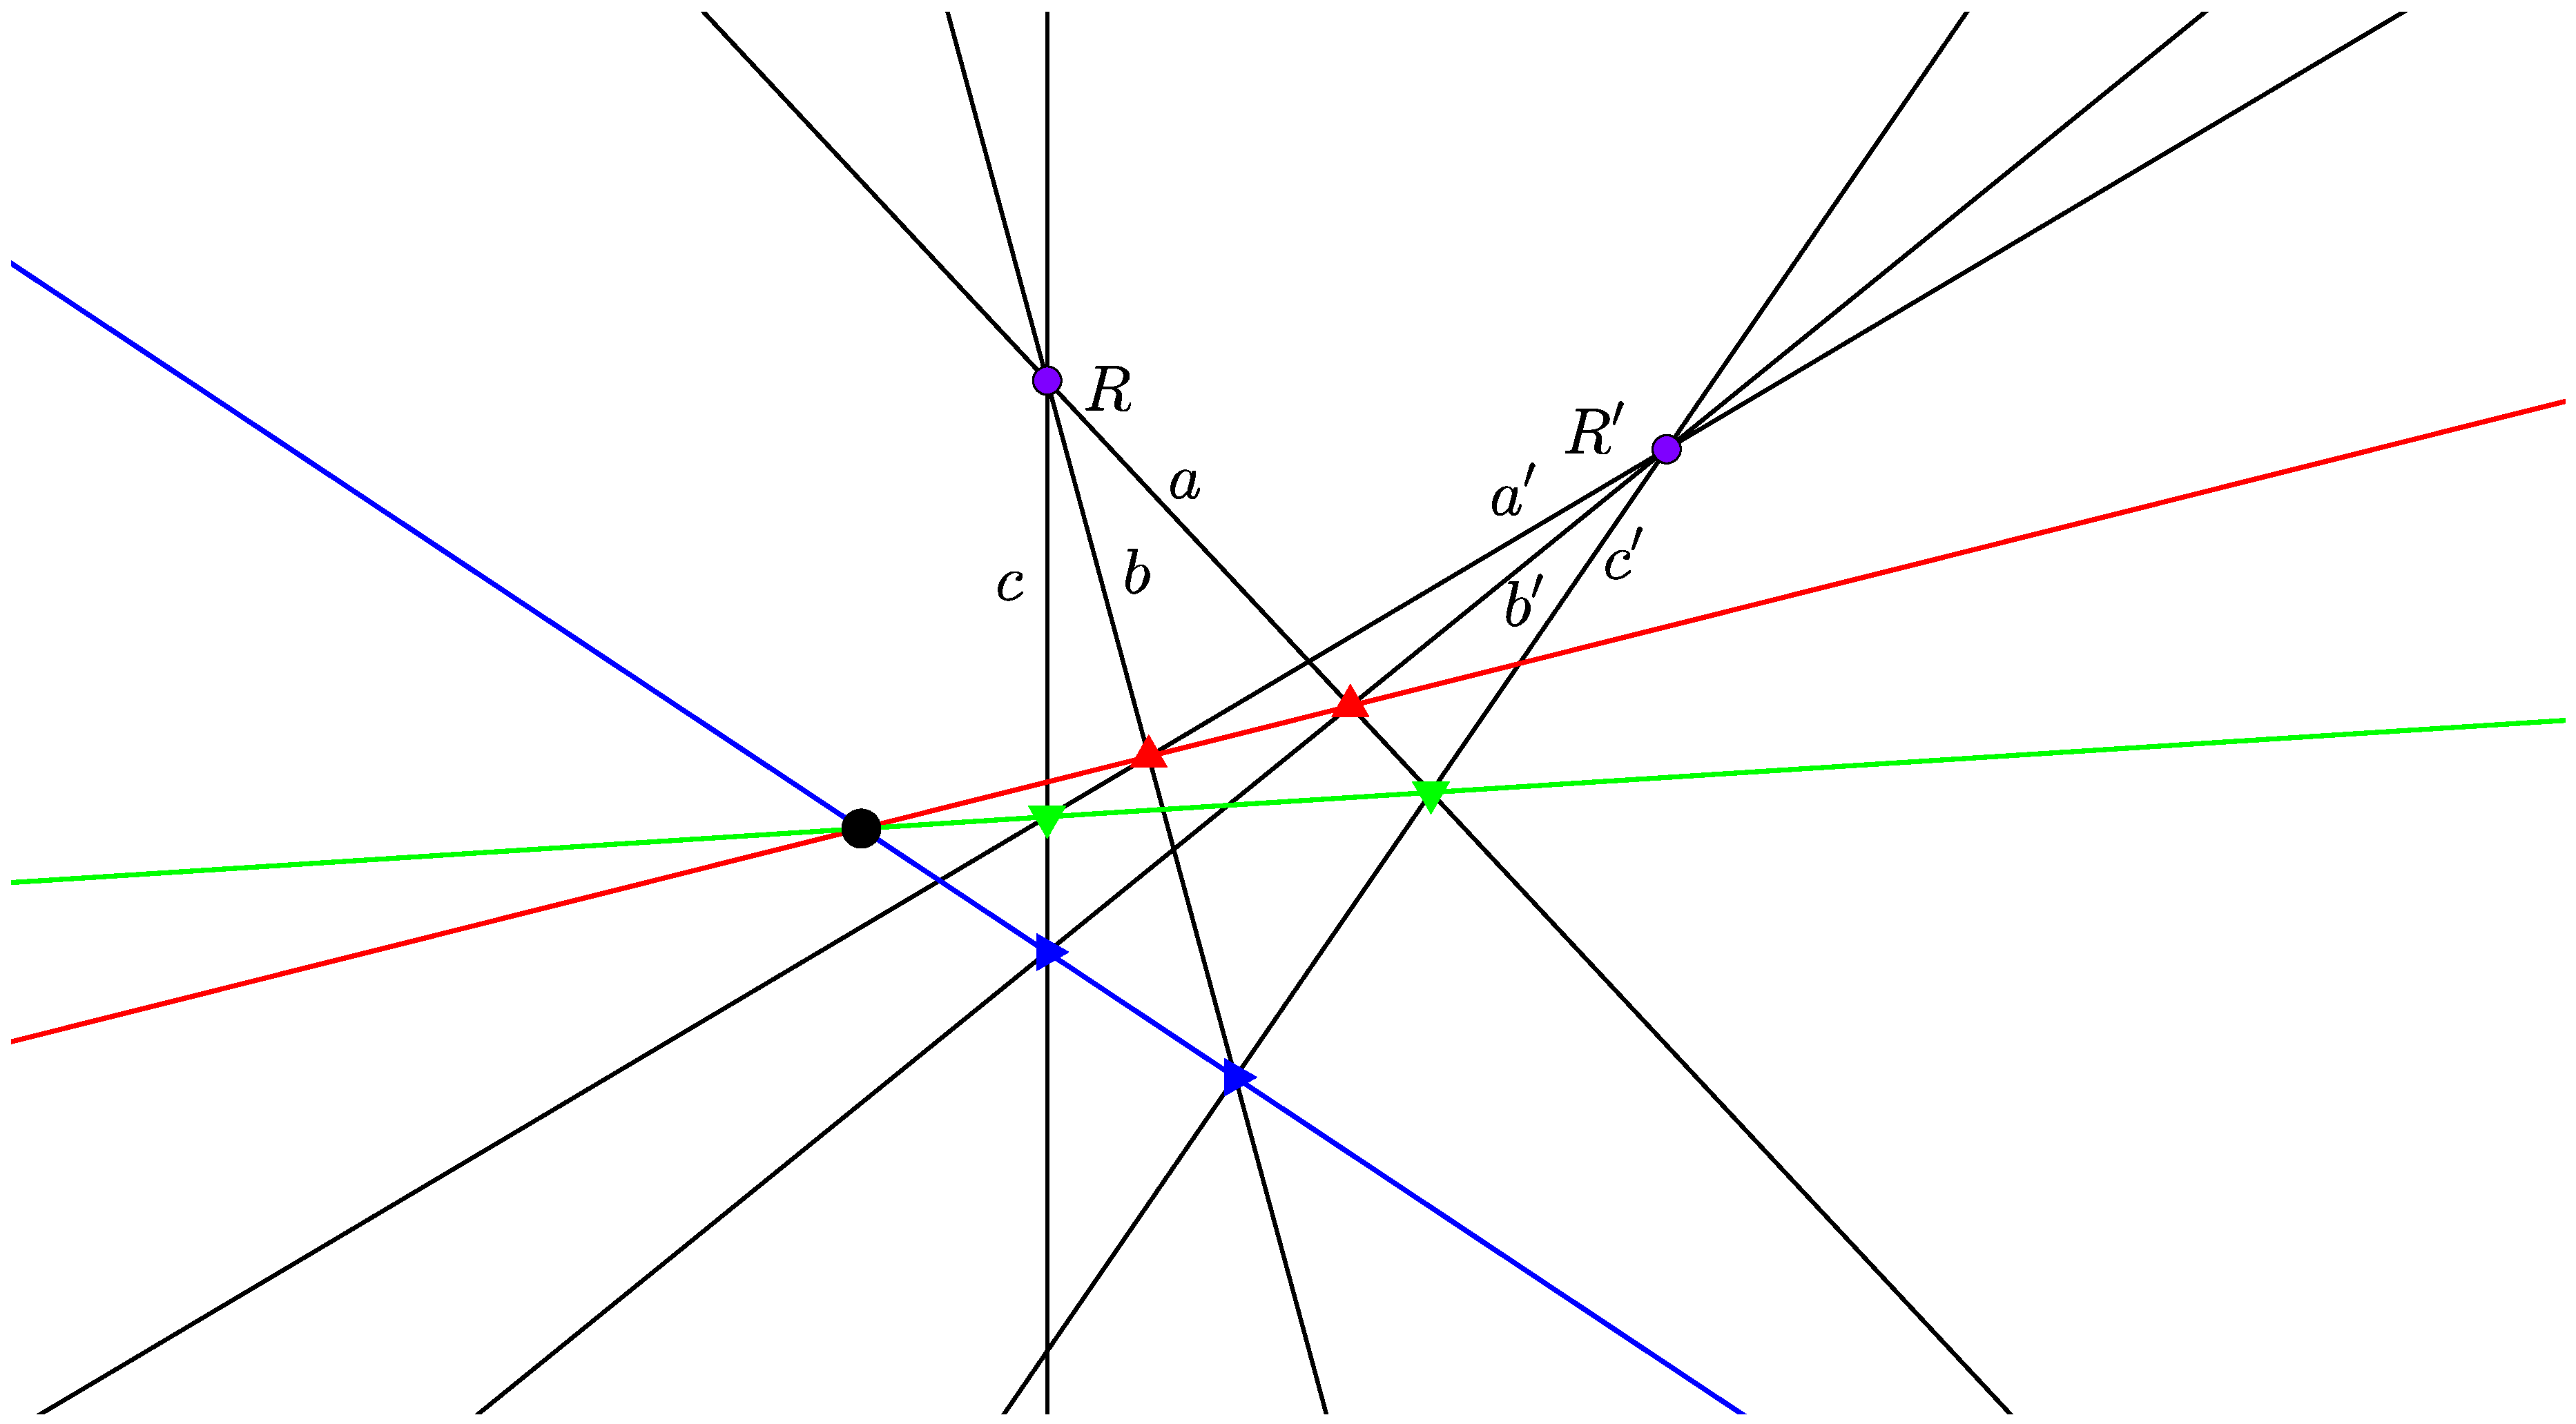
\includegraphics[scale=.25]{Graficos/DualTeoremaDePapus/Dual_Teorema_de_Papus.eps}
\end{center}
